\section{First problem}
\label{sec:p1}

A single tile is decorated with a machine which is programmed using function 
$f:[0,1] \mapsto [0,1]$. The problem \cite{exam1} claims the final graph $\Lambda$ is
a closed curve, we want to prove it first (just for fun, since this is not required).

Before doing so, we want to find the expressions of $f_1$, $f_2$ and $f_3$: respectively
the symmetrical copies of $f$ on the vertical axis, the horizontal axis and the center 
of coordinates: $O \equiv (0,0)$.
%
% Figure
%-----------------------------------------------------------
%
% One column figure
%-----------------------------------------------------------
   \begin{figure}
   \centering
\tikzstyle{smallfig}=[scale=0.25]
   %
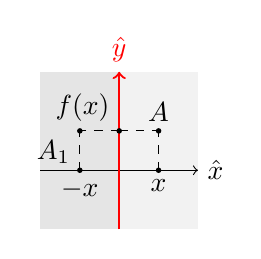
\begin{tikzpicture}[style=smallfig]
\fill [lightgray!20] (0, -3) rectangle (4, 5);
\fill [lightgray!40] (-4, -3) rectangle (0, 5);

\draw[thin,->] (-4,0) -- (4,0) node[right] {$\hat{x}$};
\draw[thick,->,red] (0,-3) -- (0,5) node[above] {$\hat{y}$};

\fill (2,2) circle (4pt) node[above] {$A$};
\draw[dashed,thin,-] (0,2.0) -- (2,2.0);
\fill (0,2) circle (4pt) node[above left] {$f(x)$};
\draw[dashed,thin,-] (2,0) node[below] {$x$} -- (2,2);
\fill (2,0) circle (4pt);
\fill (-2,2) circle (4pt) node[below left] {$A_1$};
\draw[dashed,thin,-] (0,2.0) -- (-2,2.0);
\draw[dashed,thin,-] (-2,0) node[below] {$-x$} -- (-2,2);
\fill (-2,0) circle (4pt);
\end{tikzpicture}
\quad
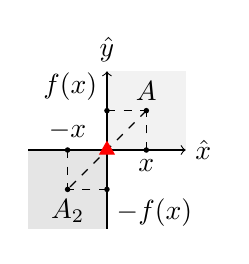
\begin{tikzpicture}[style=smallfig]
\fill [lightgray!20] (0, 0) rectangle (4, 4);
\fill [lightgray!40] (-4, -4) rectangle (0, 0);

\draw[thin,->] (-4,0) -- (4,0) node[right] {$\hat{x}$};
\draw[thin,->] (0,-4) -- (0,4) node[above] {$\hat{y}$};

\fill (2,2) circle (4pt) node[above] {$A$};
\draw[dashed,thin,-] (0,2.0) -- (2,2.0);
\fill (0,2) circle (4pt) node[above left] {$f(x)$};
\draw[dashed,thin,-] (2,0) node[below] {$x$} -- (2,2);
\fill (2,0) circle (4pt);
\fill (-2,-2) circle (4pt) node[below] {$A_2$};
\draw[dashed,thin,-] (0,-2) node[below right] {$-f(x)$} -- (-2,-2);
\draw[dashed,thin,-] (-2,0) node[above] {$-x$} -- (-2,-2);
\fill (0,-2) circle (4pt);
\draw[dashed,thin,-] (2,2) -- (-2,-2);
\fill (-2,0) circle (4pt);

\node[mark size=3pt,color=red] at (0,0) {\pgfuseplotmark{triangle*}};
\end{tikzpicture}
\quad
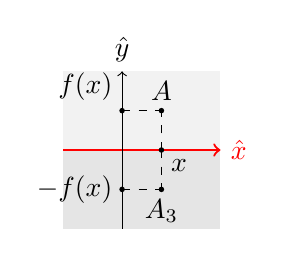
\begin{tikzpicture}[style=smallfig]
\fill [lightgray!20] (-3, 0) rectangle (5, 4);
\fill [lightgray!40] (-3, -4) rectangle (5, 0);

\draw[thick,->,red] (-3,0) -- (5,0) node[right] {$\hat{x}$};
\draw[thin,->] (0,-4) -- (0,4) node[above] {$\hat{y}$};

\fill (2,2) circle (4pt) node[above] {$A$};
\draw[dashed,thin,-] (0,2.0) -- (2,2.0);
\fill (0,2) circle (4pt) node[above left] {$f(x)$};
\draw[dashed,thin,-] (2,0) node[below right] {$x$} -- (2,2);
\fill (2,0) circle (4pt);
\fill (2,-2) circle (4pt) node[below] {$A_3$};
\draw[dashed,thin,-] (2,0) -- (2,-2);
\draw[dashed,thin,-] (0,-2) node[left] {$-f(x)$} -- (2,-2);
\fill (0,-2) circle (4pt);
\end{tikzpicture}
   %
   \caption{The three symmetrical copies of $f$. From left to
    right: vertical, center and horizontal symmetries.}
   \label{fig:symms}
   \end{figure}
%-----------------------------------------------------------
%
%-----------------------------------------------------------
%
Figure \ref{fig:symms} shows this simple calculation.

\begin{proposition}[$\Lambda$ is a closed curve]
\label{lem:lclosed}
Let $f:[0,a] \mapsto [0,a]$, with $a > 0$, be a continuous function also satisfying:
\begin{equation}
\label{eq:fconds}
f(0)=a \wedge f(a)=0 \wedge 0 \leq f(x) \leq a, \forall x \in [0,a]
\end{equation}
Then graph $\Lambda$, obtained by adjoining together $\Gamma$ ($f$'s graph) and
its vertically, horizontally and centered symmetries, is a closed curve.
\begin{proof}
Since $\Lambda$ is constructed using $\Gamma$, given that symmentry is an 
isometric\footnote{An isometry is a transformation that does not change distances and
preserves shapes.} 
transformation and that $f$ is continuous (therefore $\Gamma$ is a continuous curve
with no interruptions), then the single thing to prove is that the points were
the copies of $\Gamma$ connect with each other are continuous. We have 4
copies of $\Gamma$:
\begin{equation*}
\begin{array}{c|c|c|c}
\text{\# Quarter} & \text{\# Ranges} & \text{Graph} & \text{\# Function} \\
\hline
\text{I (NE)} & [0,a] \times [0,a] & \Gamma & f(x) \\
\text{II (NW)} & [-a,0] \times [0,a] & \Gamma_1 & f_1 = f(-x) \\
\text{III (SW)} & [-a,0] \times [-a,0] & \Gamma_2 & f_2 = -f(-x) \\
\text{IV (SE)} & [0,a] \times [-a,0] & \Gamma_3 & f_3 = -f(x) \\
\end{array}
\end{equation*}
The last column of the table shows the definitions of the symmetrical copies of $f$.
Now we can check all 4 connection points:
\begin{equation}\label{eq:symms}
\begin{array}{l|c}
f(0) = f_1(0) \implies f(0) = f(0) & ^{\Gamma}/_{\Gamma_1} \\
f_1(-a) = f_2(-a) \implies f(a) = -f(a) \implies 0 = 0 & ^{\Gamma_1}/_{\Gamma_2} \\
f_2(0) = f_3(0) \implies -f(0) = -f(0) & ^{\Gamma_2}/_{\Gamma_3} \\
f(a) = f_3(a) \implies f(a) = -f(a) \implies 0 = 0 & ^{\Gamma_3}/_{\Gamma} \\
\end{array}
\end{equation}
And that proves the thesis.
$\square$
\end{proof}
\end{proposition}

Proposition \ref{lem:lclosed} takes a generic case, but if we consider $a=1$, we
successfully get back to our case \cite{exam1}.\\

The same problem later requires to find the definition of $f$ and its symetrical
copies $f_k$ ($k = 1 \dots 3$). This task is very simple because $f$ is a line
crossing points $(1,0)$ and $(0,1)$, therefore:
\begin{equation*}
f: \frac{x-x_1}{y-y_1} = \frac{x_2-x_1}{y_2-y_1} \wedge (x_1,y_1) = (1,0), 
(x_2,y_2) = (0,1)
\end{equation*}
Which quickly leads to: $y = 1-x$, therefore: $f(x) = 1-x$. The expressions of the
copies of $f$ were found in equation \ref{eq:symms}, so by substituting $f(x)$
in $f_1$, $f_2$ and $f_3$, we find:
\begin{equation}\label{eq:exprs}
\begin{array}{l|c}
f(x) = 1 - x & \Gamma \\
f_1(x) = f(-x) \implies f_1(x) = 1 + x & \Gamma_1 \\
f_2(x) = -f(-x) \implies f_2(x) = - 1 - x & \Gamma_2 \\
f_3(x) = -f(x) \implies f_3(x) = x - 1 & \Gamma_3 \\
\end{array}
\end{equation}
This completes the first part of the problem.

\subsection{Polynomial decorations and dimensioning}
\label{sec:p1}

The next part of the problem concerns a \emph{dimensioning}\footnote{The
process of calculating the values of the parameters of a system
to reach a specic goal.} task.
The new requirements for tiles can be formalized as follows:
\begin{equation}
\label{eq:fconds2}
\begin{cases}
f^\prime(0) = 0\\
S_{\Gamma} = \gamma \cdot S \implies 
   \int^{1}_{0} f(x) \, \mathrm{d} x = \gamma \cdot S\\
\end{cases}
\end{equation}
Having $\gamma = \frac{55}{100}$ represent the fraction of area inside $\Gamma$
in relation to the whole tile, 
$S_{\Gamma} \in \mathbb{R}$ represent the surface 
inside $\Gamma$ and $S \in \mathbb{R}$ the
surface of the whole tile. The product of these two quantities is the final value 
required by the problem. 
Be carefull not to misunderstand the problem: one single tile contains one $\Gamma$,
the machine will print the other copies on 4 other different tiles. That's why the
percentage $\gamma$ does not refer to the final decoration $\Lambda$, therefore
$S = 1^2 = 1$ and $S \not\eq 2 ^ 2$. 

The problem asks to find a new function to decorate tiles and it must 
satisfy both equations \ref{eq:fconds} and \ref{eq:fconds2}.
We are suggested to use 2\textsuperscript{nd} or 3\textsuperscript{rd} 
order polynomials as the new $f$.

\begin{proposition}[2-degree polynomials don't meet conditions in equations 
\ref{eq:fconds} and \ref{eq:fconds2}]
\label{the:2degpoly}
Let $f:[0,1] \mapsto [0,1]$ be a continuous function in the form: 
$f(x) \doteq ax^2+bx+c$ where $a,b,c \in \mathbb{R}$. 
Then $f$ can never meet conditions as per both
equations \ref{eq:fconds} and \ref{eq:fconds2}.
\begin{proof}
To prove this, we need to plug $f$ inside equations \ref{eq:fconds} and 
\ref{eq:fconds2} and generate a system of equations on parameters $a$, 
$b$ and $c$:
\begin{equation*}
\begin{cases}
f(0)=1 \implies \left. ax^2+bx+c \right|_{x=0} = 1 \implies c = 1 \\
f(1)=0 \implies \left. ax^2+bx+c \right|_{x=1} = 0 \implies a+b+c=0\\
f^\prime(0) = 0 \implies \left. 2ax + b \right|_{x=0} = 0 \implies b = 0 \\
\int^{1}_{0} \left( ax^2+bx+c \right) \, \mathrm{d} x = \gamma S \\
\end{cases}
\end{equation*}
And we must also guarantee that $0 < f(x) < 1, \forall x \in [0,1]. 
$Note that the condition on continuity is observed because $f$ is a polynomial which
is continuous always. 
The first three equations define the values of the three parameters: 
$a=-1$, $b=0$ and $c=1$; which means that $f(x) = -x^2 + 1$. Let's now
verify that this function satisfies the fourth equation in the system:
\begin{align*}
&\int^{1}_{0} \left( -x^2+1 \right) \, \mathrm{d} x = \gamma S
\implies
-\int^{1}_{0} x^2 \, \mathrm{d} x + \int^{1}_{0} \mathrm{d} x = 
        \gamma S \implies \notag\\
&- \left[\frac{x^3}{3}\right]_0^1 + \left[x\right]_0^1 = \gamma S
\implies -\frac{1}{3} + 1 = \frac{55}{100} \cdot 1
\implies \frac{2}{3} = \frac{55}{100}
\end{align*}
The equation above proves that the fourth condition is the system is not met, which
proves the thesis.
$\square$
\end{proof}
\end{proposition}
Let's try with 3\textsuperscript{rd}-degree polynomials:
\begin{proposition}[3-degree polynomials meet conditions in equations 
\ref{eq:fconds} and \ref{eq:fconds2}]
\label{the:3degpoly}
Let $f:[0,1] \mapsto [0,1]$ be a continuous function in the form: 
$f(x) \doteq ax^3+bx^2+cx+d$ where $a,b,c,d \in \mathbb{R}$. 
Then $f$ meets conditions as per both
equations \ref{eq:fconds} and \ref{eq:fconds2}.
\begin{proof}
To prove this, we do as in the proof for proposition \ref{the:2degpoly}:
\begin{equation*}
\begin{cases}
f(0)=1 \implies \left. ax^3+bx^2+cx+d \right|_{x=0} = 1 \implies d = 1 \\
f(1)=0 \implies \left. ax^3+bx^2+cx+d \right|_{x=1} = 0\\
f^\prime(0) = 0 \implies \left. 3ax^2 + 2bx + c \right|_{x=0} = 0 \implies c = 0 \\
\int^{1}_{0} \left( ax^3+bx^2+cx+d \right) \, \mathrm{d} x = \gamma S \\
\end{cases}
\end{equation*}
Here as well, the condition on continuity is observed because $f$ is 
still a polynomial.
Parameters $c$ and $d$ were found, so we can re-write the system:
\begin{equation*}
\begin{cases}
\left. ax^3+bx^2+1 \right|_{x=1} = 0 \implies a+b+1=0\\
\int^{1}_{0} \left( ax^3+bx^2+1 \right) \, \mathrm{d} x = \gamma S \\
\end{cases}
\end{equation*}
Let's work on the last condition:
\begin{align*}
&\int^{1}_{0} \left( ax^3+bx^2+1 \right) \, \mathrm{d} x = \gamma S
\implies
a\int^{1}_{0} x^3 \, \mathrm{d} x + b \int^{1}_{0} x^2 \, \mathrm{d} x \, + \notag\\ 
&+ \int^{1}_{0} \mathrm{d} x= 
        \gamma S \implies 
        a \left[\frac{x^4}{4}\right]_0^1 + b \left[\frac{x^3}{3}\right]_0^1 +
        \left[x\right]_0^1 = \gamma S \implies \notag\\
&\frac{a}{4} + \frac{b}{3} + 1 = \gamma S 
\end{align*}
The final system in $a$ and $b$ can be written now as:
\begin{equation}\label{eq:3degsys}
\begin{cases}
a+b=-1\\
3a + 4b = 12 \gamma S - 12 \\
\end{cases}
\implies
\begin{pmatrix}
1 & 1 \\
3 & 4
\end{pmatrix}
\cdot
\begin{pmatrix}
a \\
b
\end{pmatrix}
=
\begin{pmatrix}
-1 \\
12 \gamma S - 12
\end{pmatrix}
\end{equation}
To verify that 3\textsuperscript{rd}-degree polynomials meet the conditions, we
just need to prove that the system in equation \ref{eq:3degsys} has a solution.
We expressed the system in matricial form to make it evident that this is a 
Cramer system\footnote{A system of $n$ linear equations in $n$ variables.},
which means that two possibilites hold: either the system has one solution only, or 
it has no solutions at all. To see which case we are in, let's calculate the determinant
of the coefficient matrix:
\begin{equation*}
\left|
\begin{matrix}
1 & 1 \\
3 & 4
\end{matrix}
\right|
= 1 \cdot 4 - 3 \cdot 1 = 4 - 3 = 1 \not\eq 0
\end{equation*}
Since the determinant is not zero, the system has one single solution, which means
that there exist values for $a$ and $b$, which together with those of $c$ and $d$ we
found before, determine a function observing equations 
\ref{eq:fconds} and \ref{eq:fconds2}.

At this point, however, our proof is not 100\% complete. We still need to prove,
as part of equation \ref{eq:fconds}, that 
$0 \leq f(x) \leq 1, \forall x \in [0,1]$; we will do this now. We start from one
important consideration: $f$ is a polynomial, it means that it is defined in all
$\mathbb{R}$ with no discontinuities. It means that:
\begin{equation*}
\not\exists x_0 \in \mathbb{R} : \lim_{x \to x_0} f(x) = \infty \wedge
\lim_{x \to \infty} f(x) = \infty
\end{equation*}
The function is a smooth curve which grows to infinity only when $x$ goes to
infinity. Which means that in $x \in [0,1]$, because of Weierstrass'
boundedness theorem, $f(x)$ has local max $M \in \mathbb{R}$ 
and min $m \in \mathbb{R}$ values. However we already know by hypothesis that
$f(0) = 1$ and $f(1) = 0$, and we want $0 \leq f(x) \leq 1$ for $0 \leq x \leq 1$;
therefore we have the following:
\begin{equation*}
m \leq 0 \leq f(x) \leq 1 \leq M, \forall x : 0 \leq x \leq 1
\end{equation*}
%
% Figure
%-----------------------------------------------------------
%
% One column figure
%-----------------------------------------------------------
   \begin{figure}
   \centering
\tikzstyle{smallfig}=[scale=0.25]
   %
\begin{tikzpicture}[style=smallfig]
\draw [fill=lightgray!20, pattern=north west lines, 
   pattern color=red] (0, 4) rectangle (4, 6);
\draw [fill=lightgray!20, pattern=north west lines, 
   pattern color=red] (4, 0) rectangle (6, 4);
\draw [fill=lightgray!20, pattern=north west lines, 
   pattern color=red] (0, -2) rectangle (4, 0);

\draw[thin,->] (-2,0) -- (6,0) node[right] {$\hat{x}$};
\draw[thin,->] (0,-2) -- (0,6) node[above] {$\hat{y}$};

\draw[dashed,thin,-] (-2,4) -- (6,4);
\draw[dashed,thin,-] (4,-2) -- (4,6);
\fill (0,4) circle (5pt) node[below left] {$1$};
\fill (4,0) circle (5pt) node[below right] {$1$};
\end{tikzpicture}
\quad
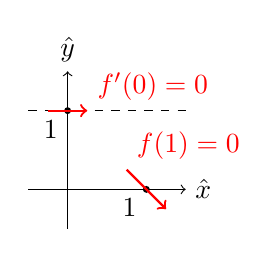
\begin{tikzpicture}[style=smallfig]
\draw[thin,->] (-2,0) -- (6,0) node[right] {$\hat{x}$};
\draw[thin,->] (0,-2) -- (0,6) node[above] {$\hat{y}$};

\draw[dashed,thin,-] (-2,4) -- (6,4);
\fill (0,4) circle (5pt) node[below left] {$1$};
\fill (4,0) circle (5pt) node[below left] {$1$};

\draw[thick,->, red] (-1,4) -- (1,4) node[above right] {$f^\prime(0)=0$};
\draw[thick,->, red] (3,1) node[above right] {$f(1)=0$} -- (5,-1);
\end{tikzpicture}
\quad
\begin{tikzpicture}[style=smallfig]
\draw[thin,->] (-2,0) -- (6,0) node[right] {$\hat{x}$};
\draw[thin,->] (0,-2) -- (0,6) node[above] {$\hat{y}$};

\fill (0,4) circle (5pt) node[below left] {$1$};
\fill (4,0) circle (5pt) node[below left] {$1$};

\begin{scope}[thick, decoration={
    markings,
    mark=at position 0.5 with {\arrow{>}}}
    ] 

    \draw[postaction={decorate}] (0,4) to[out=0,in=100] (4,0);
    \draw[postaction={decorate}] (0,4) -- (4,0);
\end{scope}
\end{tikzpicture}
   %
   \caption{Showing the how the constraints on $f$ define its shape
   in $[0,1] \times [0,1]$. The first picture shows the regione where $f$
   can lay, the middle one shows tangent in $x=0$ and the condition
   of crossing in $(1,0)$. The rightmost picture shows possible
   shapes of $f$: note how the concavity cannot be pointing upwards.}
   \label{fig:fshape}
   \end{figure}
%-----------------------------------------------------------
%
%-----------------------------------------------------------
%
This means that $m=0$ and $M = 1$. So in $x\in[0,1]$, there can only be one
relative min and one relative max. We need to prove this. Together
with the fact that $f$ is continuous, we basically need to prove that $f$ is
monotonically decreasing inside $[0,1]$ like figure \ref{fig:fshape} shows. To
prove this, we must study $f$'s monotonicity: the most classic way to do this
is by considering its first-order derivative $f^\prime$ and verify that
$f^\prime(x) < 0, \forall x \in ]0,1[$.
$\square$
\end{proof}
\end{proposition}
We are asked to find the values of $a$, $b$, $c$ and $d$ though. Since $c=0$ and
$d=1$, we need to calculate $a$ and $b$ from equation \ref{eq:3degsys}.
We simple rearrange the matricial equation multiplying both members by the
inverse of the coefficient matrix (on the left side of course):
\begin{align*}
&
\begin{pmatrix}
1 & 1 \\
3 & 4
\end{pmatrix}^{-1}
\cdot
\begin{pmatrix}
1 & 1 \\
3 & 4
\end{pmatrix}
\cdot
\begin{pmatrix}
a \\
b
\end{pmatrix}
=
\begin{pmatrix}
1 & 1 \\
3 & 4
\end{pmatrix}^{-1}
\cdot
\begin{pmatrix}
-1 \\
12 \gamma S - 12
\end{pmatrix}
\implies \notag\\
&\begin{pmatrix}
a \\
b
\end{pmatrix}
=
\begin{pmatrix}
1 & 1 \\
3 & 4
\end{pmatrix}^{-1}
\cdot
\begin{pmatrix}
-1 \\
12 \gamma S - 12
\end{pmatrix}
\end{align*}
Let's calculate the inverse of the coefficient matrix:
\begin{align*}
&
\begin{pmatrix}
1 & 1 \\
3 & 4
\end{pmatrix}^{-1}
=
\begin{bmatrix}
(-1)^{1+1}C_{1,1} & (-1)^{1+2}C_{1,2} \\
(-1)^{2+1}C_{2,1} & (-1)^{2+2}C_{2,2}
\end{bmatrix}^\text{T}
= \notag\\
&=\begin{bmatrix}
(-1)^{1+1} \cdot 4 & (-1)^{1+2} \cdot 3 \\
(-1)^{2+1} \cdot 1 & (-1)^{2+2} \cdot 1
\end{bmatrix}^\text{T}
=
\begin{pmatrix}
4 & -3 \\
-1 & 1
\end{pmatrix}^\text{T}
=
\begin{pmatrix}
4 & -1 \\
-3 & 1
\end{pmatrix}
\end{align*}
So, we can now calculate $a$ and $b$:
\begin{equation*}
\begin{pmatrix}
a \\
b
\end{pmatrix}
=
\begin{pmatrix}
4 & -1 \\
-3 & 1
\end{pmatrix}
\cdot
\begin{pmatrix}
-1 \\
12 \gamma S - 12
\end{pmatrix}
=
\begin{pmatrix}
-4 +12 -12 \gamma S \\
3 - 12 + 12 \gamma S
\end{pmatrix}
\end{equation*}
Considering that $12 \gamma S = 12 \cdot \frac{55}{100} \cdot 1 = \frac{66}{10}$,
we have that $a = 8 - \frac{66}{10} = \frac{7}{5}$, and 
$b = -9 + \frac{66}{10} = -\frac{12}{5}$.